% ============================================================
% Reporte tecnico: Analisis Exploratorio de Datos
% Proyecto: Deteccion de Neumonia - RSNA Pneumonia Detection Challenge
% Maestria en Ciencia de Datos / Inteligencia Artificial
% Autor: [Nombre del estudiante]
% Fecha: Marzo 2026
% ============================================================
\documentclass[11pt,spanish]{article}

% --- Codificacion y fuentes ---
\usepackage[utf8]{inputenc}
\usepackage[T1]{fontenc}
\usepackage{lmodern}

% --- Idioma ---
\usepackage[spanish,es-nodecimaldot]{babel}

% --- Geometría: márgenes APA-like en carta ---
\usepackage[letterpaper, top=2.54cm, bottom=2.54cm,
            left=3cm, right=2.5cm]{geometry}

% --- Tablas ---
\usepackage{booktabs}
\usepackage{array}
\usepackage{tabularx}
\usepackage{multirow}

% --- Figuras ---
\usepackage{graphicx}
\usepackage{float}
\usepackage[labelfont=bf, labelsep=period, font=small]{caption}
\usepackage{subcaption}

% --- Espaciado y párrafos ---
\usepackage{parskip}
\setlength{\parskip}{6pt}
\setlength{\parindent}{0pt}

% --- Colores y líneas de regla ---
\usepackage{xcolor}
\usepackage{titlesec}

% --- Formato de secciones ---
\titleformat{\section}{\normalfont\bfseries\large}{}{0em}{}[\titlerule]
\titleformat{\subsection}{\normalfont\bfseries}{}{0em}{}

% --- Interlineado 1.15 ---
\usepackage{setspace}
\setstretch{1.15}

% --- Ruta de figuras ---
\graphicspath{{salida_eda/}}

% ============================================================
\begin{document}

% ----------------------------------------------------------
% ENCABEZADO
% ----------------------------------------------------------
\begin{center}
  {\LARGE\bfseries Análisis Exploratorio de Datos}\\[4pt]
  {\large Conjunto RSNA Pneumonia Detection Challenge}\\[6pt]
  {\normalsize Reporte técnico --- Actividad de análisis exploratorio}\\[2pt]
  {\small Marzo de 2026}
\end{center}

\vspace{0.3cm}
\hrule
\vspace{0.4cm}

% ----------------------------------------------------------
% 1. RESULTADOS DEL PREPROCESAMIENTO
% ----------------------------------------------------------
\section{Resumen del procesamiento previo}

A partir del conjunto de datos público \textit{RSNA Pneumonia Detection Challenge} se ejecutó
un pipeline de preprocesamiento que integró tres fuentes de información: las imágenes
radiológicas en formato DICOM del conjunto de entrenamiento, el archivo de etiquetas
\texttt{stage\_2\_train\_labels.csv} y el archivo de clases detalladas
\texttt{stage\_2\_detailed\_class\_info.csv}.

Las transformaciones realizadas fueron: (1)~verificación de integridad de los 26\,684 archivos
DICOM del split de entrenamiento —ningún archivo resultó corrupto o ilegible—;
(2)~integración de ambas tablas CSV mediante la llave \textit{patientId}, resultando en 37\,629
registros a nivel de anotación; (3)~construcción de una variable binaria de diagnóstico
(\textit{target\_binaria}: 0 = negativo, 1 = positivo); (4)~validación geométrica de las
cajas delimitadoras (\textit{bounding boxes}) para casos positivos —todas resultaron válidas
dentro de las dimensiones de sus imágenes—; y (5)~partición estratificada en tres subconjuntos:
entrenamiento (70\,\%), validación (15\,\%) y prueba (15\,\%), conservando la proporción
de clases en cada partición.

La \textbf{base final depurada} quedó conformada por \textbf{26\,684 pacientes válidos}:
6\,012 positivos (22.53\,\%) y 20\,672 negativos (77.47\,\%), distribuidos en 18\,678 registros
de entrenamiento, 4\,003 de validación y 4\,003 de prueba.

% ----------------------------------------------------------
% 2. GRÁFICOS UNIVARIANTES
% ----------------------------------------------------------
\section{Gráficos univariantes}

\subsection{Distribución de clases clínicas}

La Figura~\ref{fig:clases} muestra la distribución de frecuencias de las tres categorías
clínicas del conjunto. La categoría \textit{No Lung Opacity / Not Normal} es la más frecuente,
con 11\,821 registros (44.30\,\%), seguida de \textit{Normal} con 8\,851 (33.17\,\%) y
\textit{Lung Opacity} con 6\,012 (22.53\,\%). Esta distribución evidencia un desbalance
de clases que deberá considerarse en las etapas de modelado; en particular, los casos positivos
representan menos de la cuarta parte del total.

\begin{figure}[H]
  \centering
  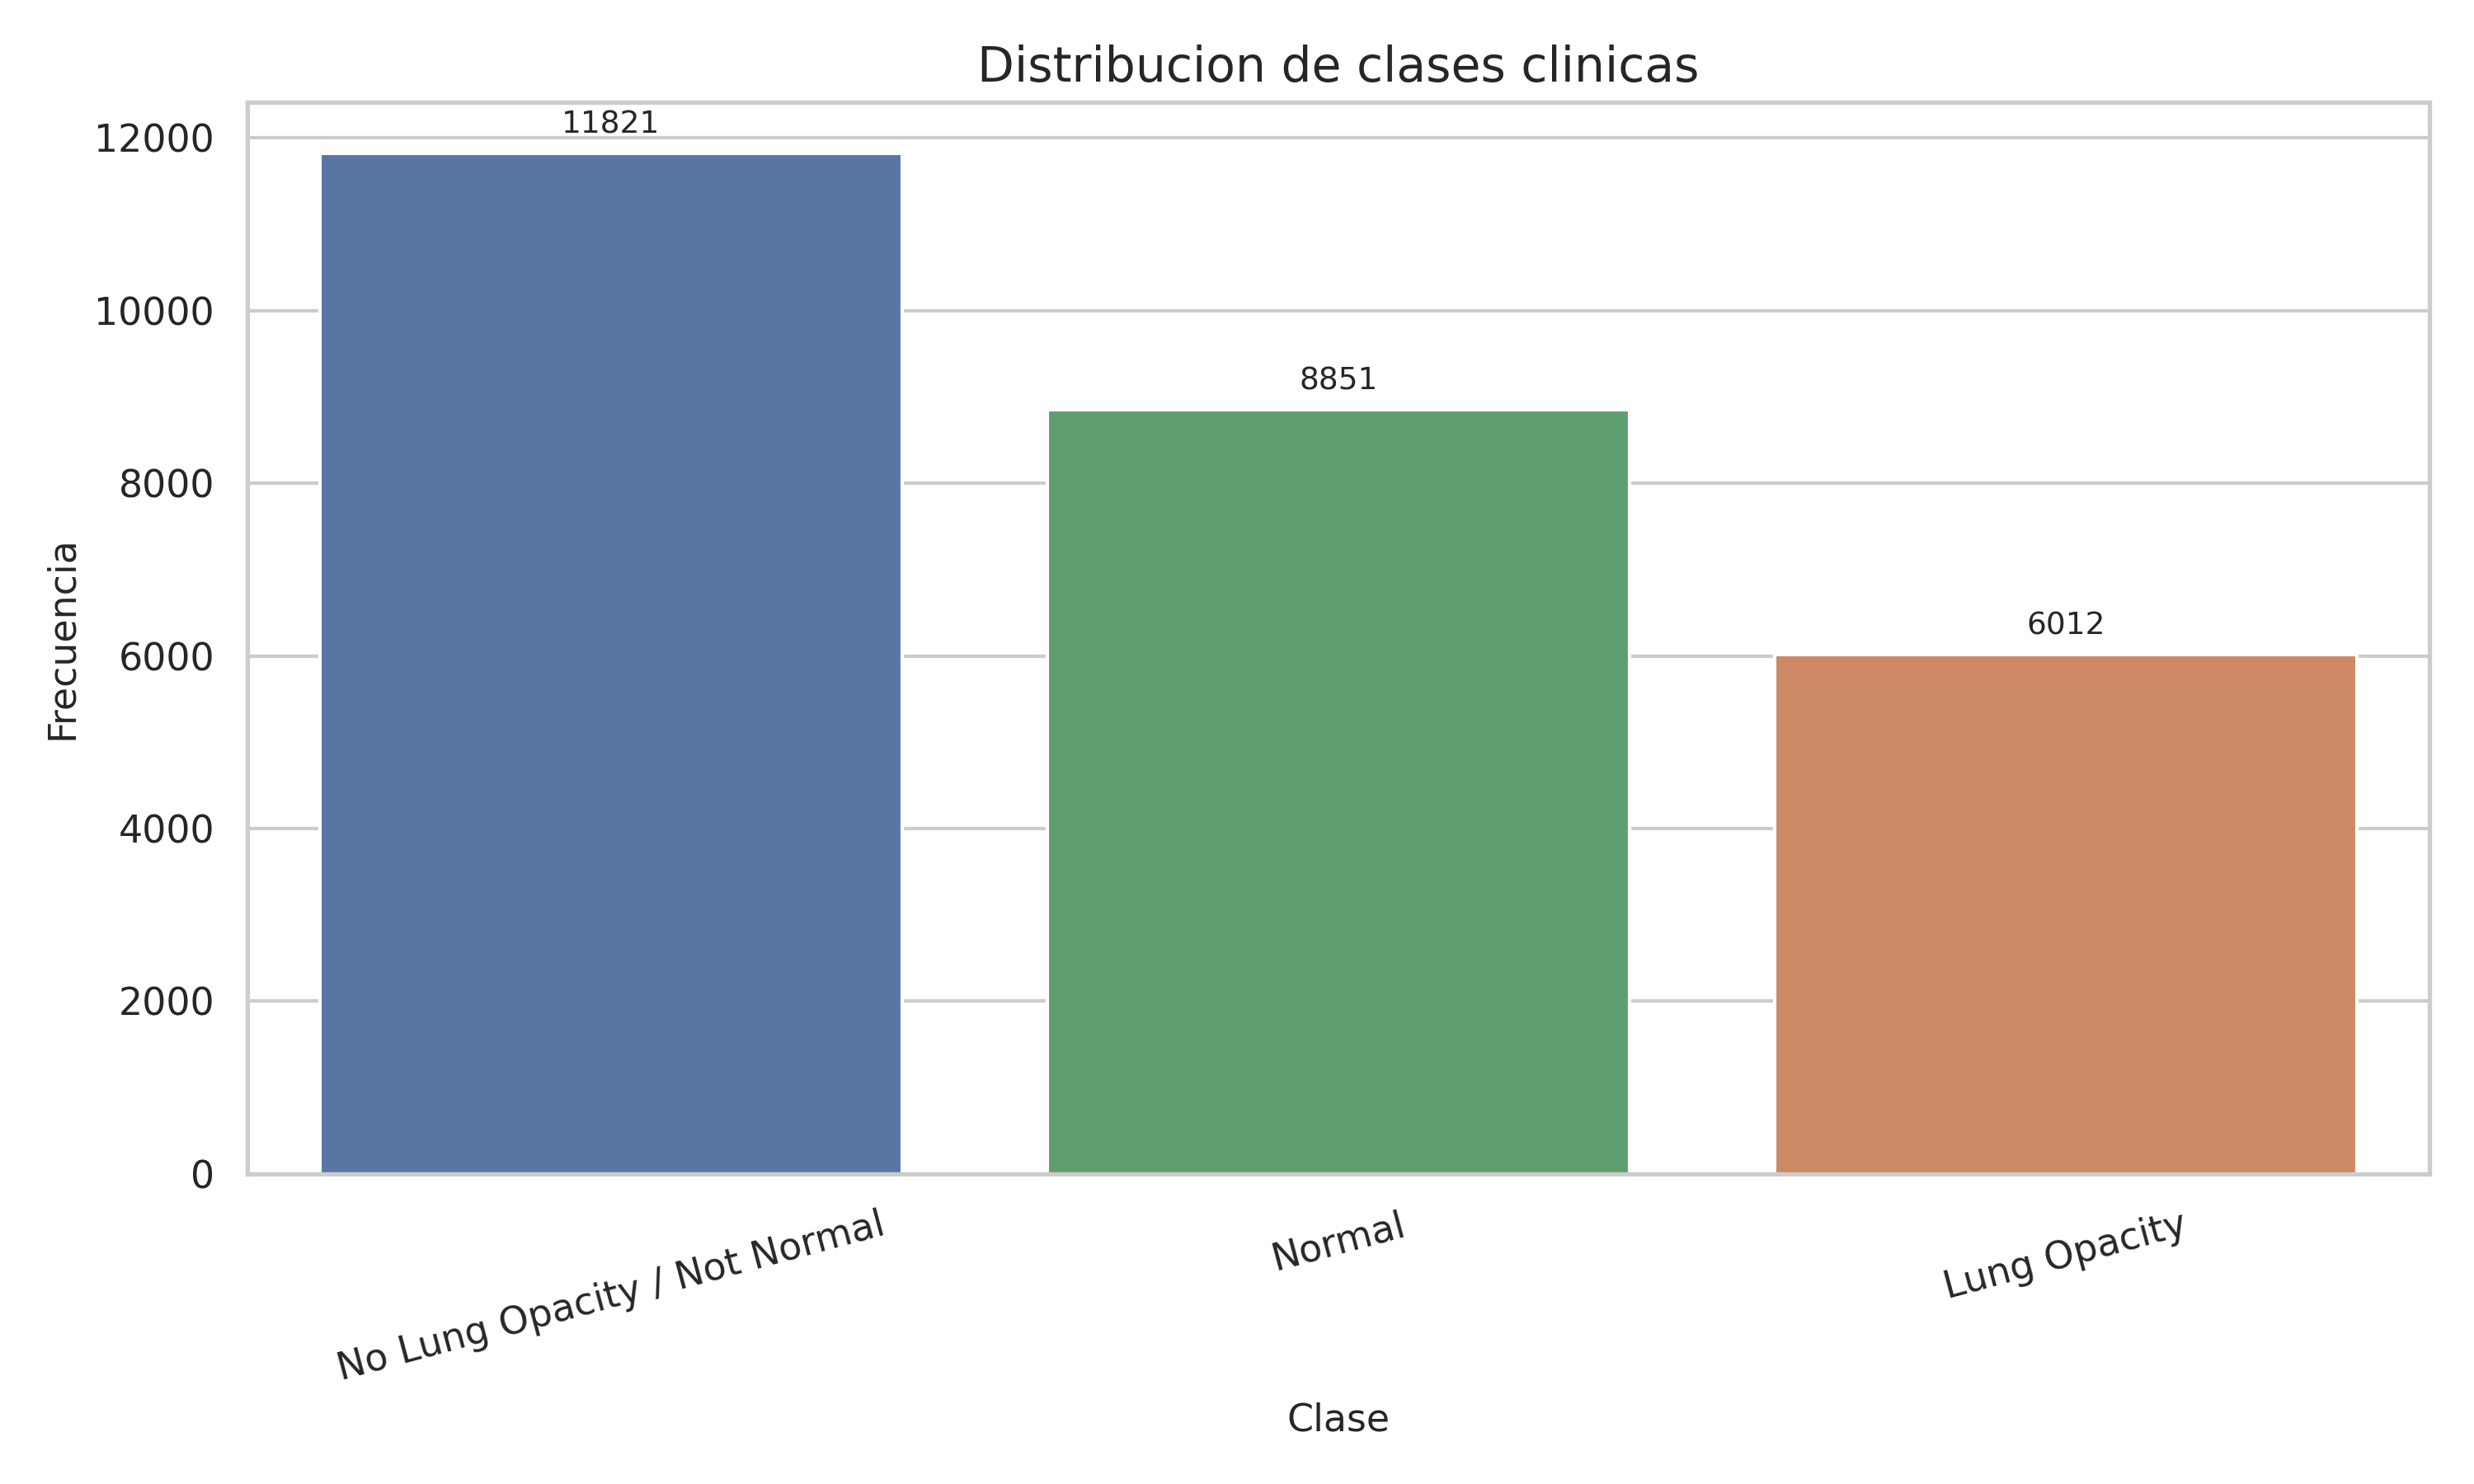
\includegraphics[width=0.72\textwidth]{grafico_univariante_clases.png}
  \caption{Distribución de frecuencias por clase clínica. Las barras muestran el conteo
           absoluto de pacientes por categoría en el conjunto depurado ($n = 26\,684$).}
  \label{fig:clases}
\end{figure}

\subsection{Distribución del área total de bounding boxes en casos positivos}

La Figura~\ref{fig:bbox_area} presenta el histograma del área total de las cajas
delimitadoras en los 6\,012 casos positivos. La distribución es marcadamente asimétrica
hacia la derecha: la mayoría de los pacientes tienen áreas de lesión relativamente pequeñas,
mientras que una minoría presenta opacidades de gran extensión. Este comportamiento sugiere
heterogeneidad clínica en la gravedad de las lesiones.

\begin{figure}[H]
  \centering
  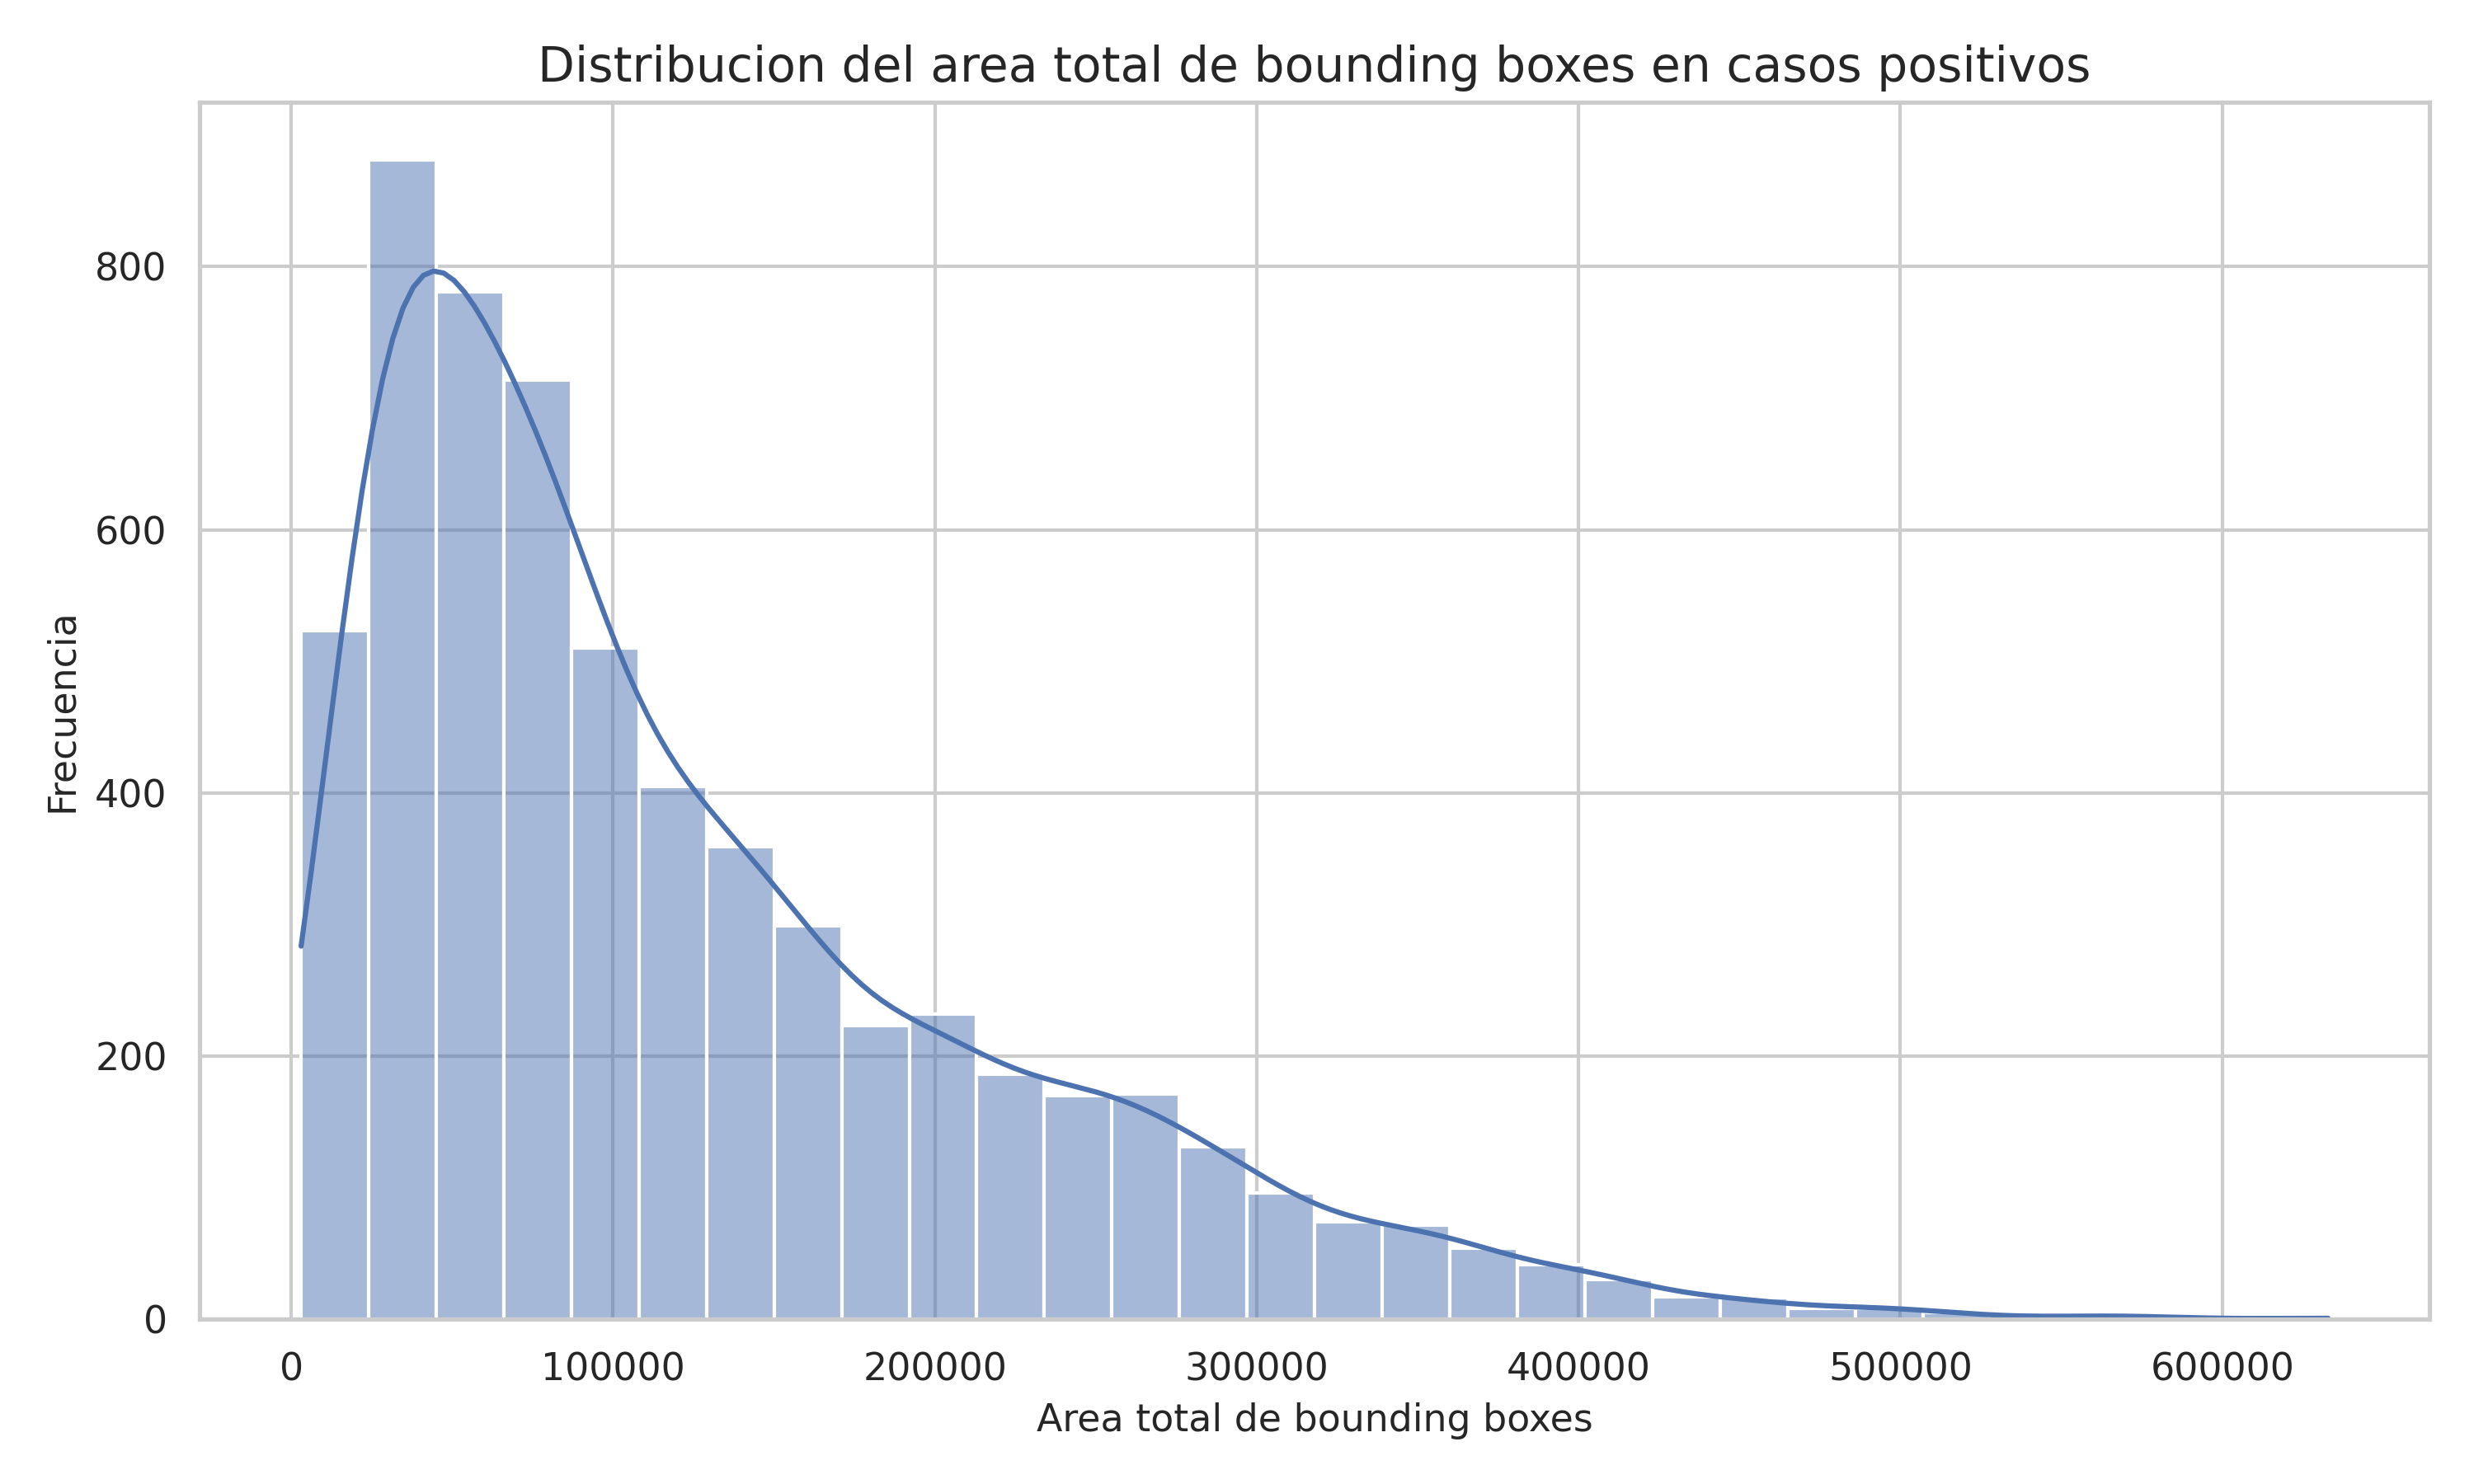
\includegraphics[width=0.72\textwidth]{grafico_univariante_area_bbox.png}
  \caption{Histograma del área total de \textit{bounding boxes} en casos positivos
           ($n = 6\,012$). La línea continua representa la densidad estimada mediante
           un kernel gaussiano.}
  \label{fig:bbox_area}
\end{figure}

% ----------------------------------------------------------
% 3. GRÁFICOS MULTIVARIANTES
% ----------------------------------------------------------
\section{Gráficos multivariantes}

\subsection{Distribución de casos por partición y clase binaria}

La Figura~\ref{fig:split_target} confirma que la estratificación de la partición se realizó
correctamente: en los tres subconjuntos (train, val, test) la proporción de positivos y
negativos se mantiene aproximadamente igual, lo que garantiza que los modelos sean evaluados
bajo condiciones representativas de la distribución original.

\begin{figure}[H]
  \centering
  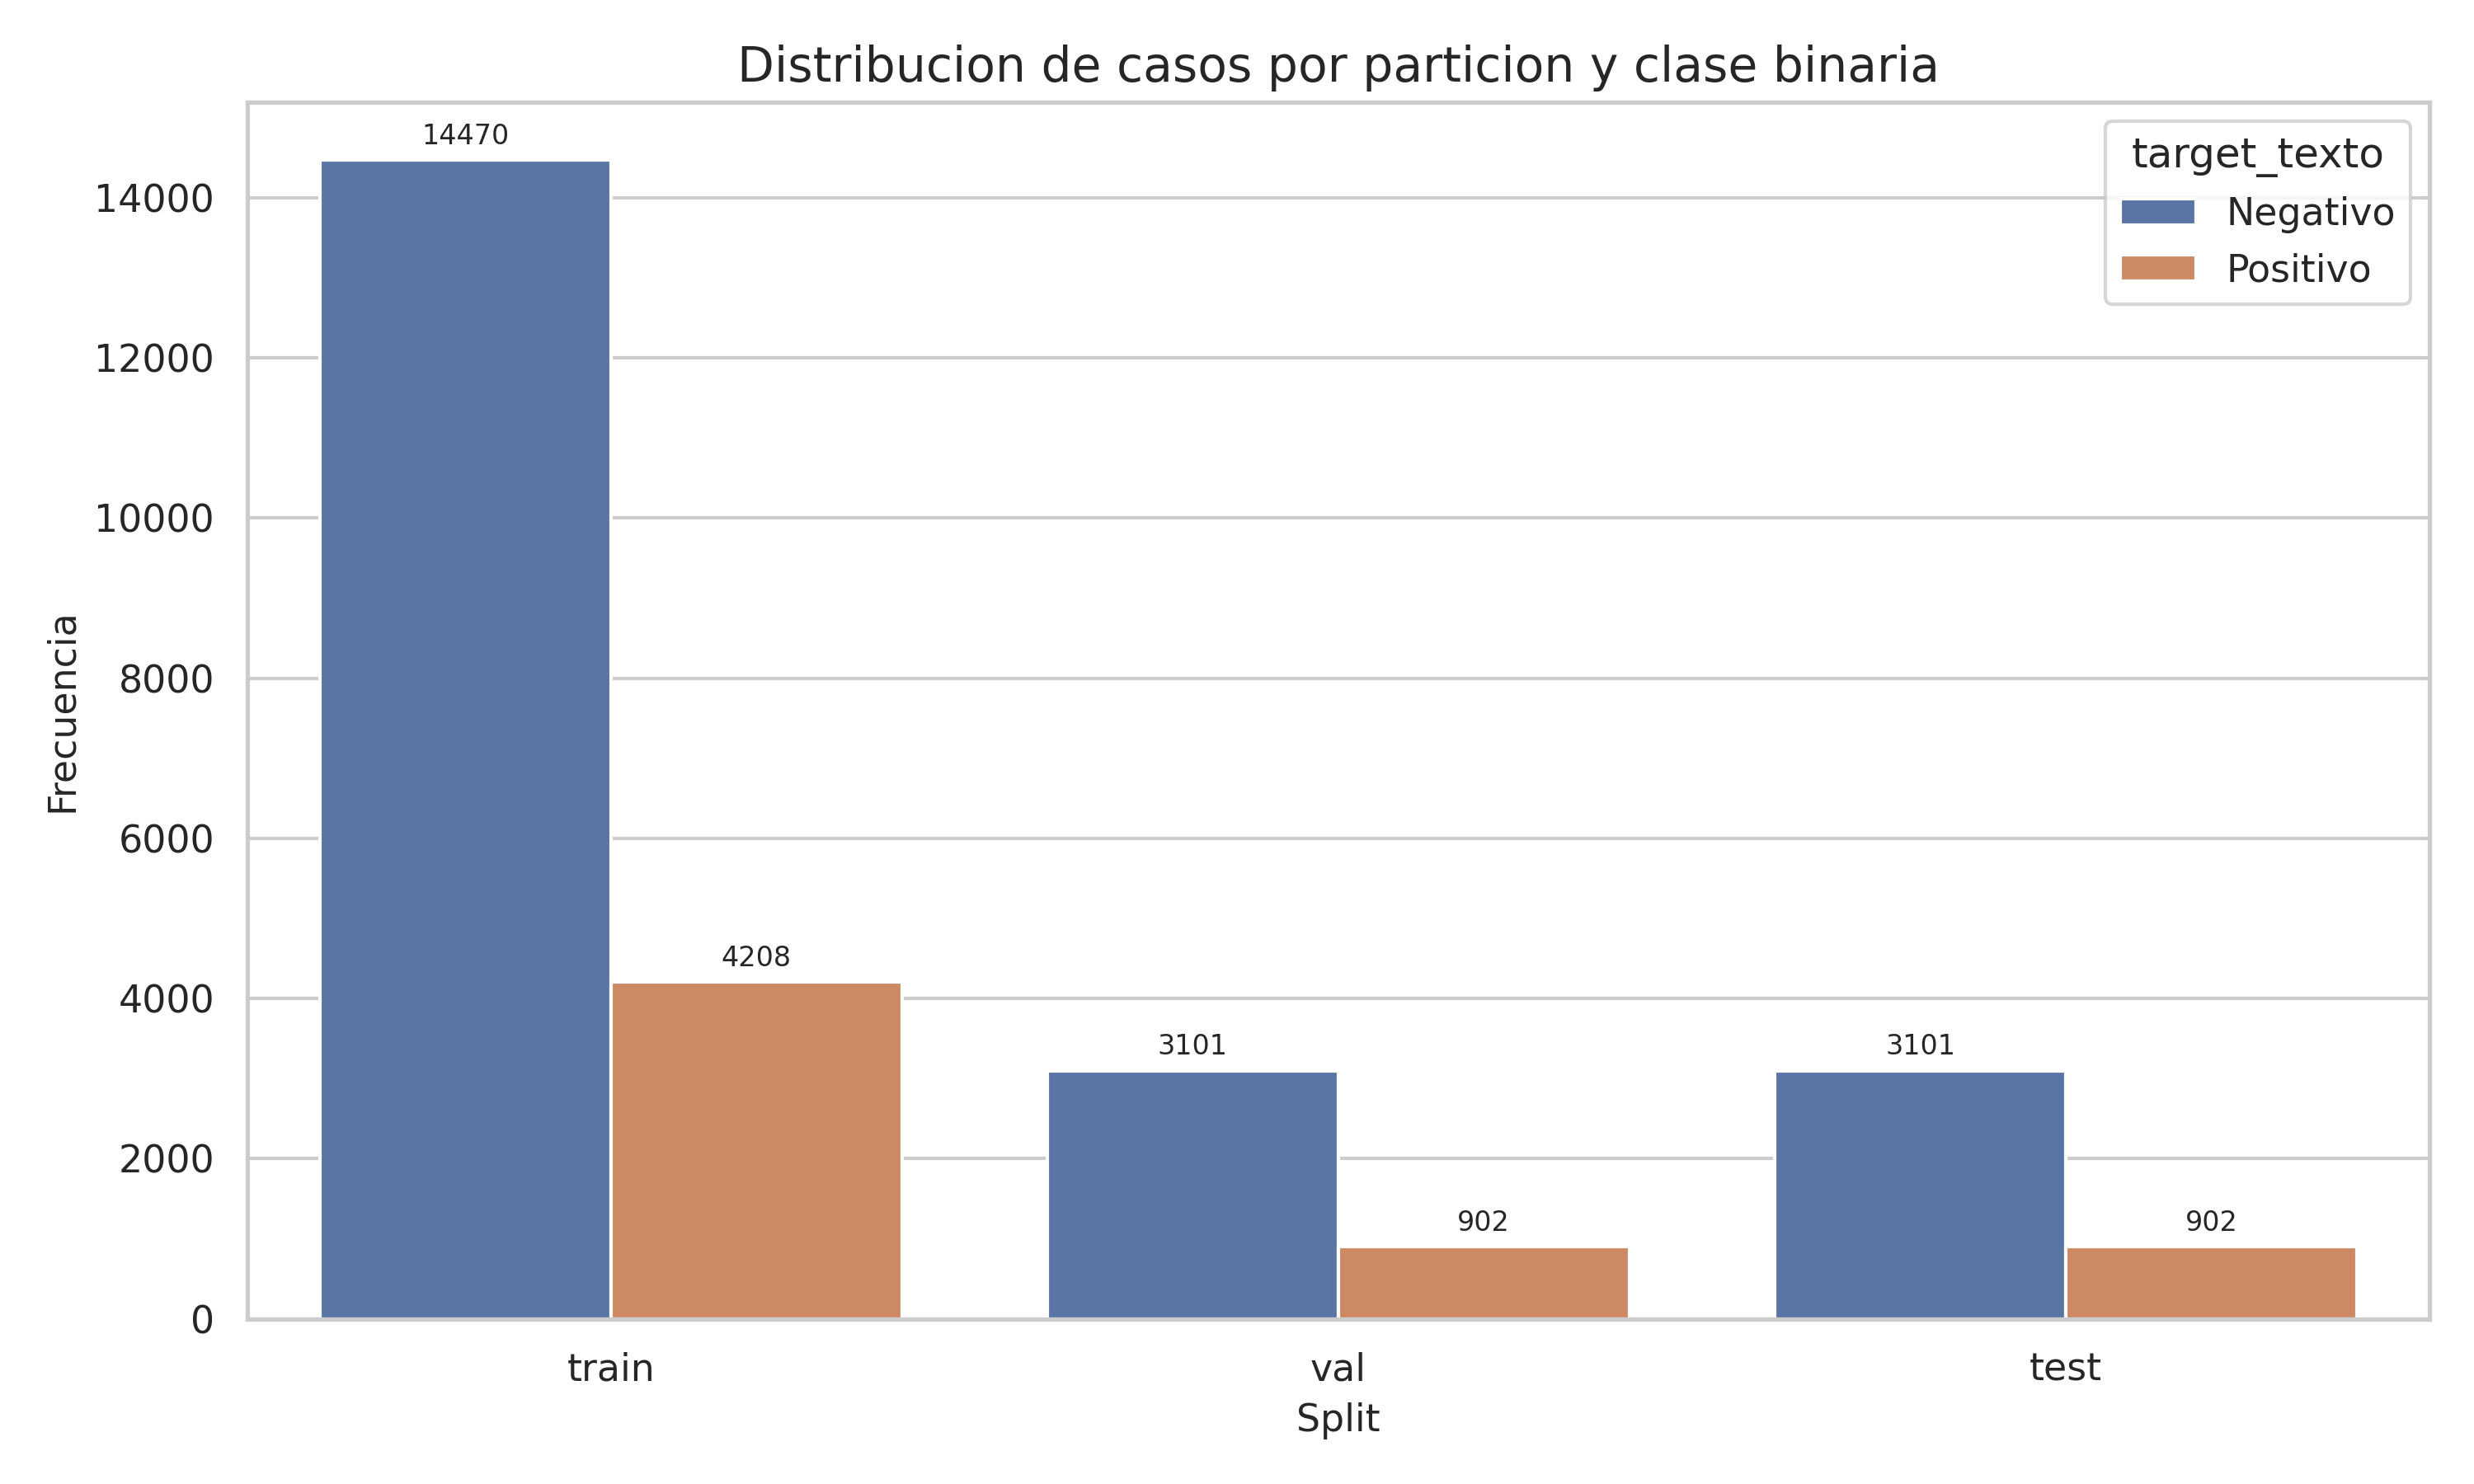
\includegraphics[width=0.72\textwidth]{grafico_multivariante_split_target.png}
  \caption{Frecuencia de casos positivos y negativos por subconjunto de datos
           (train / val / test). Los números sobre las barras indican el conteo absoluto.}
  \label{fig:split_target}
\end{figure}

\subsection{Mapa de calor de correlaciones}

La Figura~\ref{fig:corr} presenta la matriz de correlaciones de Pearson entre la variable
objetivo y las métricas derivadas de las cajas delimitadoras. Se observa alta correlación
entre \textit{bbox\_area\_total} y las demás dimensiones geométricas, lo cual es esperado
dado que el área es función del ancho y del alto. La variable \textit{target\_binaria}
correlaciona de forma notable con todas las métricas de caja, corroborando que sólo los casos
positivos poseen anotaciones espaciales.

\begin{figure}[H]
  \centering
  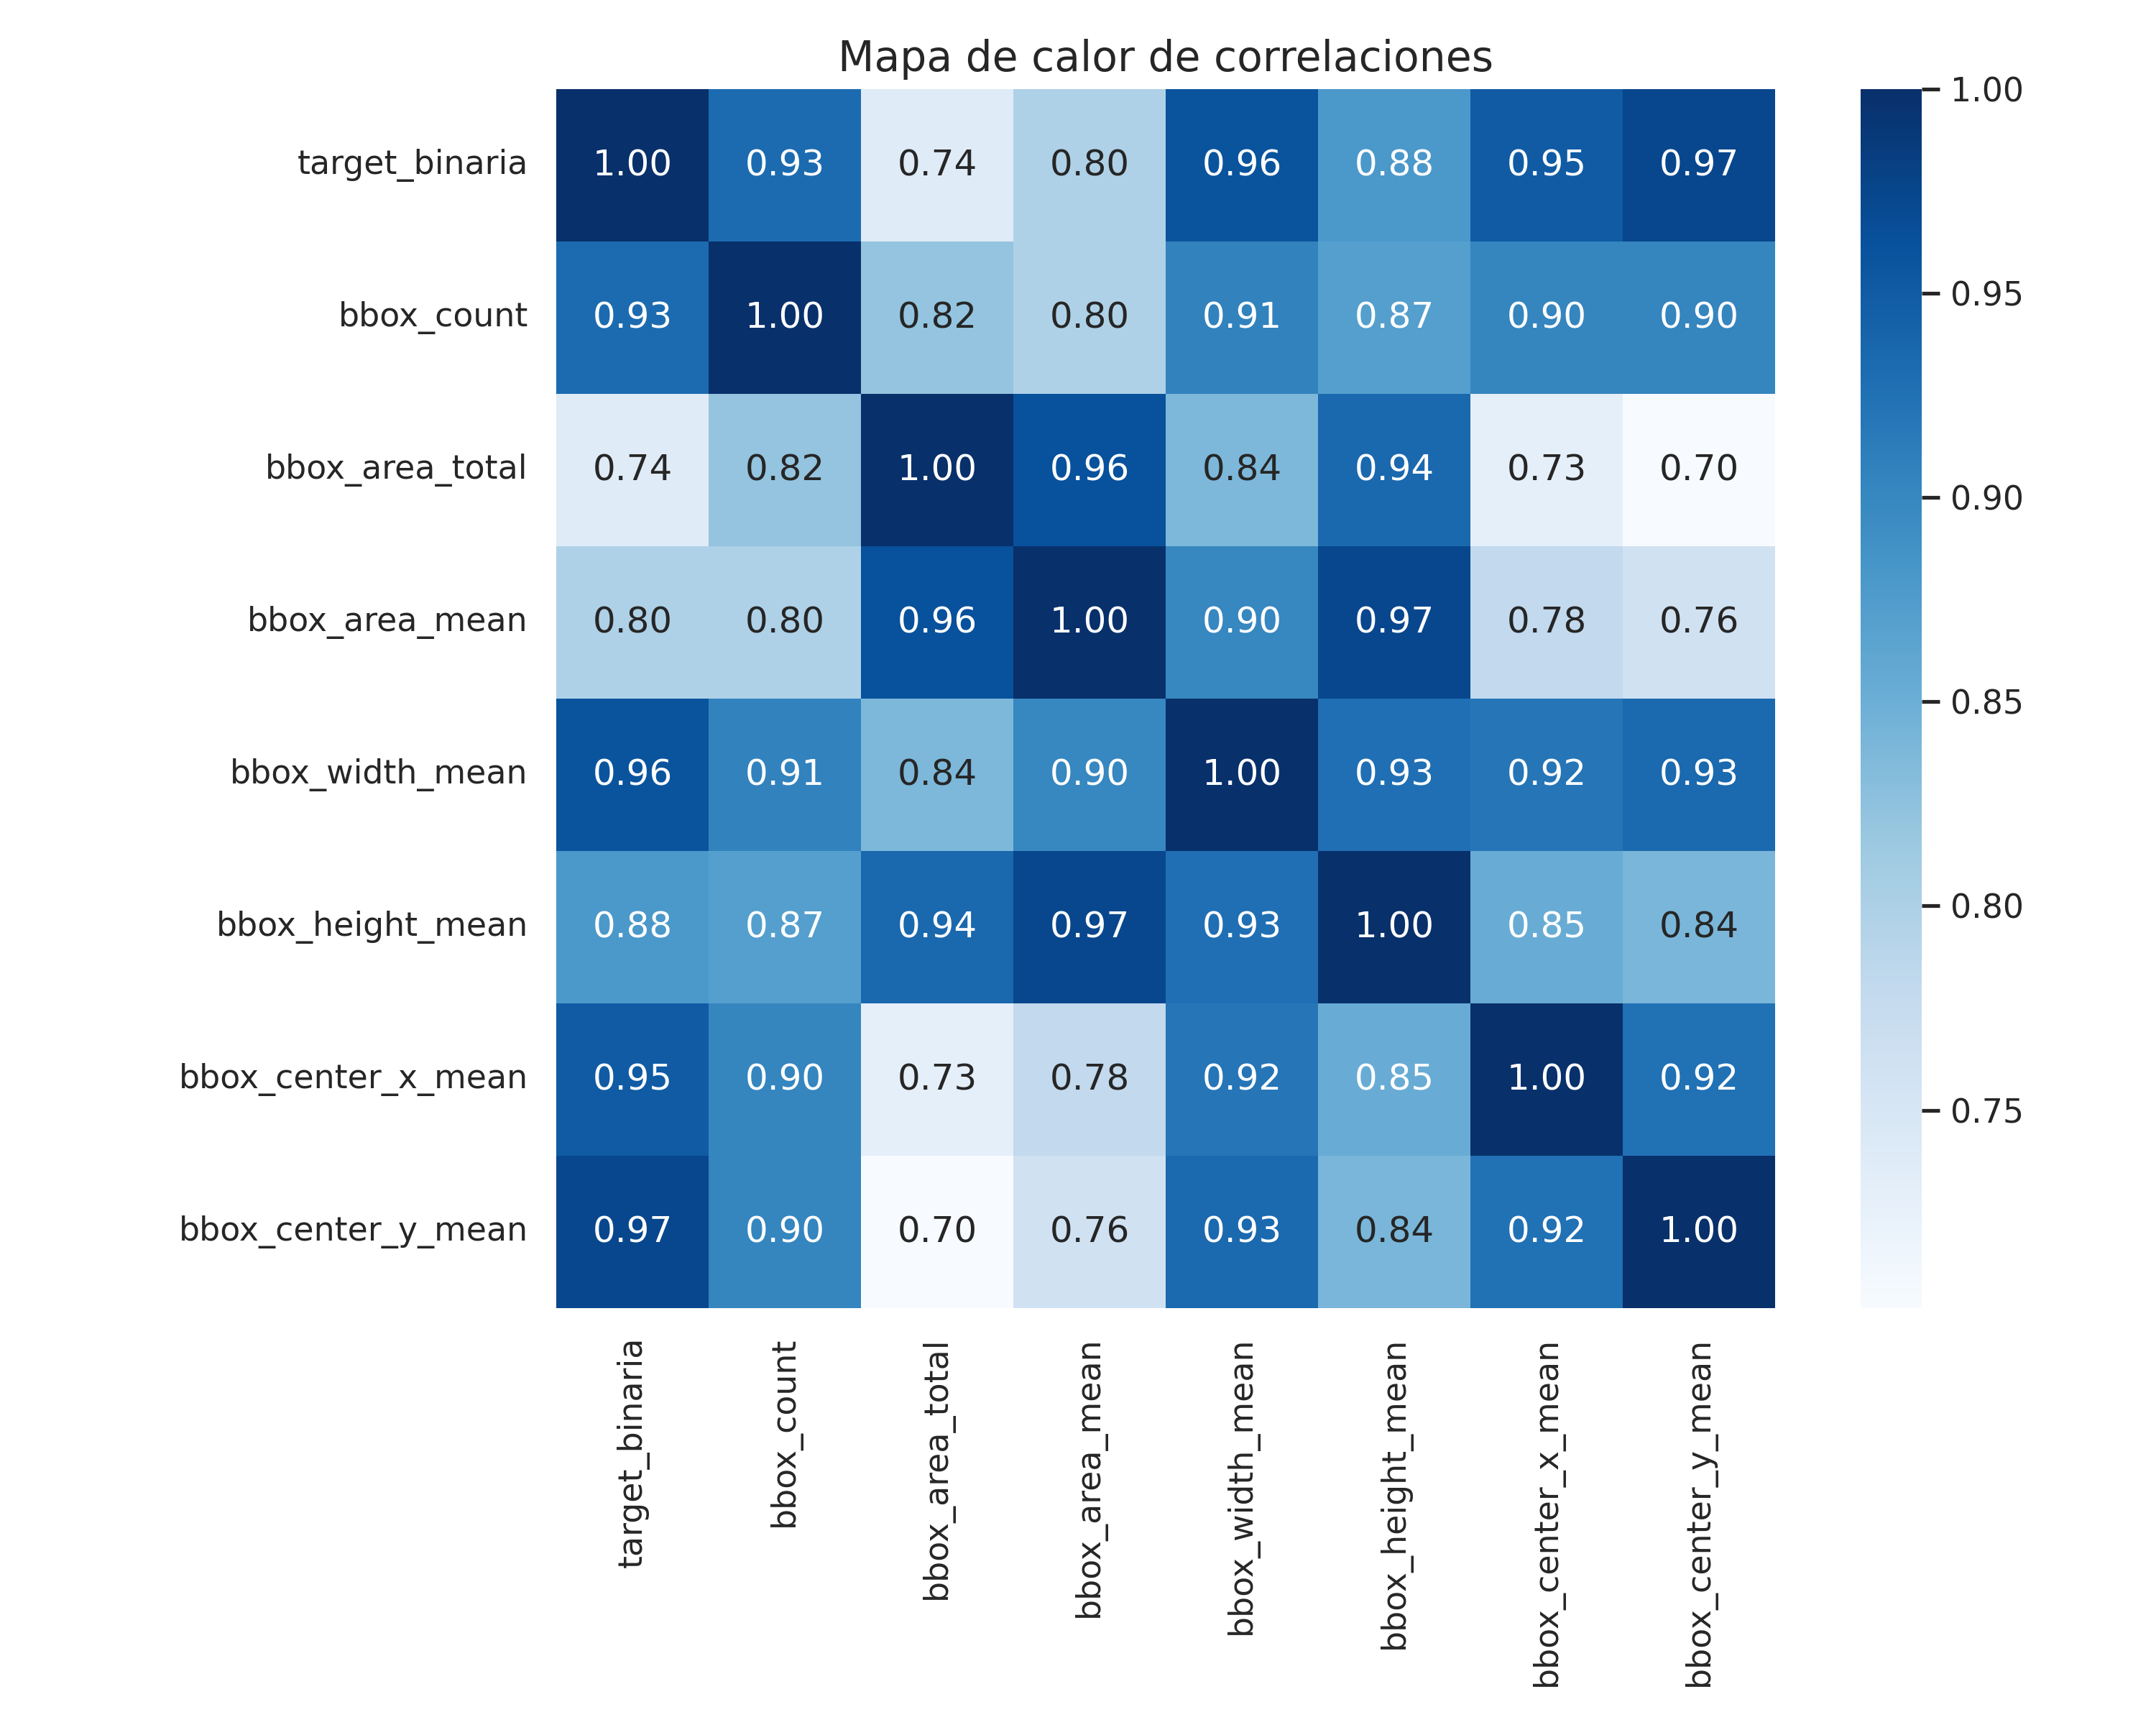
\includegraphics[width=0.72\textwidth]{grafico_multivariante_correlaciones.png}
  \caption{Mapa de calor de correlaciones de Pearson entre variables numéricas del
           conjunto EDA. Los valores mostrados en cada celda representan el coeficiente
           de correlación redondeado a dos decimales.}
  \label{fig:corr}
\end{figure}

% ----------------------------------------------------------
% 4. RESÚMENES ESTADÍSTICOS
% ----------------------------------------------------------
\section{Resúmenes estadísticos}

El Cuadro~\ref{tab:estadisticos} presenta las medidas de tendencia central y dispersión
para las principales variables numéricas del conjunto. La media de \textit{target\_binaria}
(0.2253) confirma la prevalencia de aproximadamente una en cuatro observaciones como positivo.
Las métricas de áreas muestran medianas de cero —reflejo de que el 77.47\,\% de los registros
no tienen anotación— y desviaciones estándar elevadas, lo que indica alta variabilidad entre
los casos positivos.

\begin{table}[H]
\centering
\small
\caption{Resumen estadístico de las variables numéricas del conjunto depurado ($n = 26\,684$).
         Las métricas de caja (\textit{bbox}) son válidas para todos los registros;
         los negativos tienen valor cero al no poseer anotaciones.}
\label{tab:estadisticos}
\begin{tabular}{lccccc}
\toprule
\textbf{Variable} & \textbf{Media} & \textbf{Mediana} & \textbf{Mín.} & \textbf{Máx.} & \textbf{D.E.} \\
\midrule
\textit{target\_binaria}     & 0.2253  & 0.00   & 0.00 & 1.00      & 0.4178  \\
\textit{bbox\_count}          & 0.3581  & 0.00   & 0.00 & 4.00      & 0.7122  \\
\textit{bbox\_area\_total}    & 27\,759.58 & 0.00 & 0.00 & 632\,892.00 & 69\,708.91 \\
\textit{bbox\_area\_mean}     & 16\,522.06 & 0.00 & 0.00 & 371\,184.00 & 38\,411.06 \\
\textit{bbox\_width\_mean}    & 48.71   & 0.00   & 0.00 & 528.00    & 94.22  \\
\textit{bbox\_height\_mean}   & 70.76   & 0.00   & 0.00 & 904.50    & 149.19 \\
\bottomrule
\end{tabular}
\end{table}

El Cuadro~\ref{tab:grupo} compara los indicadores de caja entre grupos. Los 6\,012 pacientes
positivos presentan en promedio 1.59 cajas por estudio y un área total media de 123\,209.67
píxeles cuadrados, con mediana de 91\,651.50 —menor a la media, lo que confirma la asimetría
observada en el histograma—. Los negativos no poseen anotaciones, de manera que todos sus
indicadores son cero.

\begin{table}[H]
\centering
\small
\caption{Estadísticos de área de \textit{bounding boxes} por grupo diagnóstico.}
\label{tab:grupo}
\begin{tabular}{lrrrr}
\toprule
\textbf{Grupo} & \textbf{Pacientes} & \textbf{Proporción}
               & \textbf{Área total (media)} & \textbf{Área total (mediana)} \\
\midrule
Negativo & 20\,672 & 77.47\,\% & 0.00       & 0.00 \\
Positivo &  6\,012 & 22.53\,\% & 123\,209.67 & 91\,651.50 \\
\bottomrule
\end{tabular}
\end{table}

% ----------------------------------------------------------
% 5. HALLAZGO CLAVE
% ----------------------------------------------------------
\section{Hallazgo principal del análisis exploratorio}

El hallazgo más relevante de este análisis es la \textbf{coexistencia de desbalance de clases
y variabilidad espacial intraclase}. La clase positiva (\textit{Lung Opacity}) representa
únicamente el 22.53\,\% del conjunto, pero cada paciente positivo contiene en promedio 1.59
lesiones anotadas, con áreas que van desde valores muy pequeños hasta 632\,892 píxeles
cuadrados. Esto significa que el problema no es sólo de clasificación binaria, sino que también
involucra localización e identificación de regiones con extensión variable. Estas características
implican que las estrategias de modelado deberán contemplar técnicas de
\textit{oversampling}, ponderación de clases o pérdidas adaptativas para compensar el
desbalance, así como arquitecturas capaces de manejar la heterogeneidad espacial de las lesiones.

\end{document}
